

\def\ifundefined#1{\expandafter\ifx\csname#1\endcsname\relax}
\ifundefined{inputGnumericTable}
	\def\gnumericTableEnd{\end{document}}
\documentclass[Journal,11pt,twocolumn]{IEEEtran}
\usepackage{tabularx}
\usepackage{tikz}
\usetikzlibrary{shapes,arrows}
\usepackage{circuitikz}
  \usepackage[latin1]{inputenc}                                 %%
    \usepackage{color}                                            %%
    \usepackage{array}                                            %%
    \usepackage{longtable}                                        %%
    \usepackage{calc}                                             %%
    \usepackage{multirow}                                         %%
    \usepackage{hhline}                                           %%
    \usepackage{ifthen}   
    \usepackage{listings}
    \usepackage{hyperref}
\usepackage{amsmath,amssymb}
 \makeatletter
\newsavebox\myboxA
\newsavebox\myboxB
\newlength\mylenA
\newcommand*\xoverline[2][0.75]{%
    \sbox{\myboxA}{$\m@th#2$}%
    \setbox\myboxB\null% Phantom box
    \ht\myboxB=\ht\myboxA%
    \dp\myboxB=\dp\myboxA%
    \wd\myboxB=#1\wd\myboxA% Scale phantom
    \sbox\myboxB{$\m@th\overline{\copy\myboxB}$}%  Overlined phantom
    \setlength\mylenA{\the\wd\myboxA}%   calc width diff
    \addtolength\mylenA{-\the\wd\myboxB}%
    \ifdim\wd\myboxB<\wd\myboxA%
       \rlap{\hskip 0.5\mylenA\usebox\myboxB}{\usebox\myboxA}%
    \else
        \hskip -0.5\mylenA\rlap{\usebox\myboxA}{\hskip 0.5\mylenA\usebox\myboxB}%
    \fi}
\makeatother

\begin{document}

\title{ASSEMBL
Y-Assignment}
\author{Adarsh kumar (FWC2022068)}
\maketitle
\begin{abstract}
This manual will explain how to design a 4-Bit Synchronous Counter Using 7474 IC
\end{abstract}
\IEEEpeerreviewmaketitle
\section{\textbf{Components Needed}}
\begin{tabularx}{0.5\textwidth} {  
  | >{\centering\arraybackslash}X  
  | >{\centering\arraybackslash}X  
  | >{\centering\arraybackslash}X |}
  \hline
\textbf{Component} &  \textbf{Value} & \textbf{Quantity}\\
\hline
Arduino & Uno & 1 \\  
\hline
Resistor & 220ohm & 1 \\ 
\hline
Bread board & - & 1 \\
\hline
Jumper wires & M-M & 20\\
\hline
Seven segment Display & Common Anode & 1\\
\hline
Decoder & 7447 & 1\\
\hline
Flip Flop & 7474 & 2\\
\hline
\end{tabularx}
\section{\textbf{7447 IC Pin Diagram}}
\begin{tikzpicture}[scale=1.1,
     pin/.style={draw,rectangle,minimum width=2em,font=\small}
     ]
   % Main trick: loop over the label numbers and then adjust their position
   % in the tikzpicture using evaluate to calculate \y=y-coordinate of pin

   \foreach \i/\desc [evaluate=\i  as \x using (\i+4.8 )]
      in {1/\tiny{B},
          2/\tiny{C},
          3/\tiny{\xoverline{LT}},
          4/\tiny{\xoverline{BI/RBO}},
          5/\tiny{\xoverline{RBI}},
          6/\tiny{D},
          7/\tiny{A},
          8/\tiny{GND}}
   {
     \draw node[pin,anchor=east,rotate=360] at (\x,-0.233){\small$\i$};
     \node[align=right,anchor=east,rotate=360] at (\x,-.8){\desc};
   }
  
   \foreach \i/\desc [evaluate=\i as \x using (21.1-\i)]
      in { 9/\xoverline{e},
          10/\xoverline{d},
          11/\xoverline{c},
          12/\xoverline{b},
          13/\xoverline{a},
          14/\xoverline{g},
          15/\xoverline{f},
          16/{V$_{\text{CC}}$}}
   {
     \draw node[pin,anchor=west,rotate=360] at (\x,3.22){\small$\i$};
     \node[align=right,anchor=west,rotate=360] at (\x,3.8){\desc};
   }
   \draw
      (5,0.8)--(5,3)--(5,3)--(13,3)--(13,3)
             --(13,0.8)--(13,0)--(5,0)--cycle;
    \begin{scope}         
    \clip (15,.5) rectangle (5,2);         
   \draw(5.2,1.5)circle[radius=0.3];
   \end{scope}
   \begin{scope}
   \clip (18,-1.5) rectangle (15,1);
    \draw (2,) circle(6.5);
\end{scope}

   \node at (9,1.5){\textbf{\LARGE{7447}}};
 \end{tikzpicture}
\section{\textbf{7474 IC Pin Diagram}}
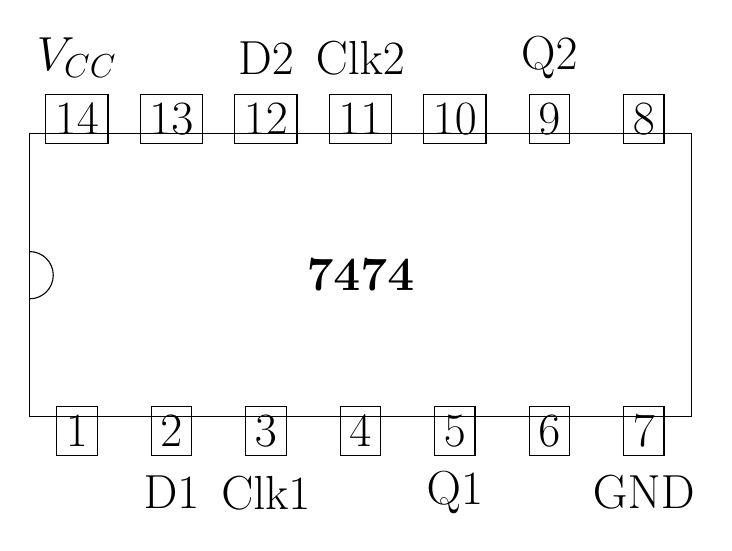
\begin{tikzpicture}[scale=0.6,
     pin/.style={draw,rectangle,minimum width=0.3em,font=\small}
     ]
%   \clip (18,.5) rectangle (3,1);           
%Vertices of the main display rectangle
\def \xmin{0}
\def \xmax{12}
\def \ymin{0}
\def \ymax{6}

%Number of pins on a side
\def \n{7}
\def \k{1.6}

%Draw the display rectangle


%Define height of pins and their separation
\def \height{1}
\pgfmathsetmacro{\centx}{(\xmax+\xmin)/2}
\pgfmathsetmacro{\centy}{(\ymax+\ymin)/2}
\pgfmathsetmacro{\wid}{(\xmax-\xmin)/(\n-1)}


\draw ({\xmin-0.5*\wid},\ymin)rectangle ({\xmax+0.5*\wid},\ymax);

%Defining y axis divisions
\pgfmathsetmacro{\ywid}{(\ymin-\ymax)/(\n-2)}

%Putting text 7447 at the centre
   \node at (\centx,\centy) {\textbf{\LARGE{7474}}};

      
\foreach [count=\i] \k in {$V_{CC}$,,D2,Clk2,,Q2,}
   {
\pgfmathsetmacro{\j}{int(round(15-\i)}
\draw node[pin,anchor=center] at ({\xmin+(\i-1)*\wid},{\ymin-0.15*\wid}){\LARGE \i};
\draw node[pin,anchor=center] at ({\xmin+(\i-1)*\wid},{\ymax+0.15*\wid}){\LARGE \j};
            \node (\i) at ( {\xmin+(\i-1)*\wid},{\ymax+0.8*\wid}) {\LARGE \k} ;
   }

\foreach [count=\i] \k in {,D1,Clk1,,Q1,,GND}
{
            \node (\i) at ( {\xmin+(\i-1)*\wid},{\ymin-0.8*\wid}) {\LARGE \k} ;              
 }
\draw (-0.5*\wid,{\centy-0.5}) arc (-90:90:0.5) ;
\end{tikzpicture}

\section{\textbf{Seven Segment Display Pinout}}
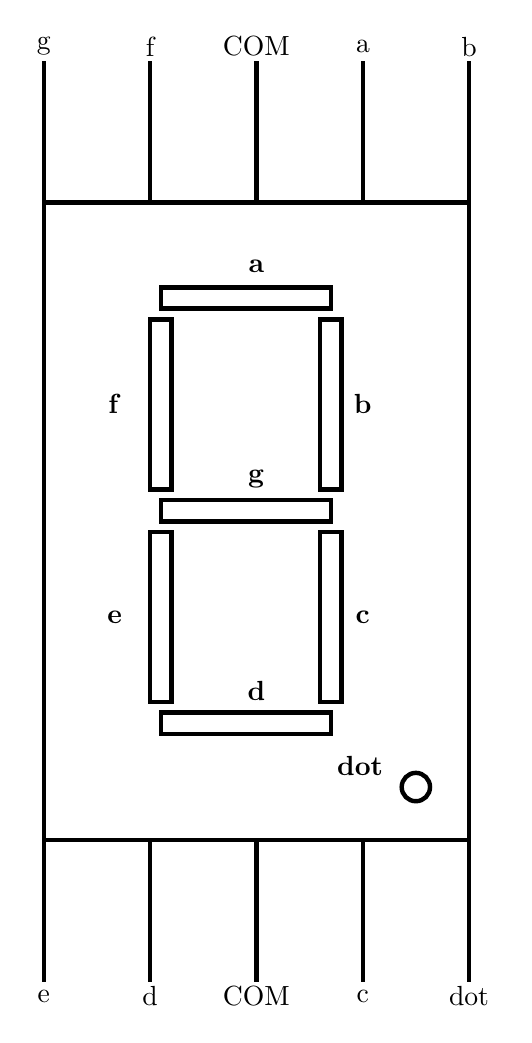
\begin{tikzpicture}
  [
    scale=0.9,
    >=stealth,
    point/.style = {draw, circle,  fill = black, inner sep = 0.5pt},
    dot/.style   = {draw, circle,  fill = black, inner sep = .2pt},
  ]

%Vertices of the main display rectangle
\def \xmin{0}
\def \xmax{6}
\def \ymin{0}
\def \ymax{-9}

%Number of pins on a side
\def \n{5}
\def \k{1.6}

%Draw the display rectangle
\draw[ultra thick] (\xmin,\ymin)rectangle (\xmax,\ymax);

%Define height of pins and their separation
\def \height{2}
\pgfmathsetmacro{\wid}{(\xmax-\xmin)/(\n-1)}

%Defining y axis divisions
\pgfmathsetmacro{\ywid}{(\ymin-\ymax)/(\n-2)}

\foreach \i in {0,...,4}
{
\draw[ultra thick] (\xmin + \i*\wid, \ymin) -- (\xmin + \i*\wid, \ymin + \height); 
\draw[ultra thick] (\xmin + \i*\wid, \ymax) -- (\xmin + \i*\wid, \ymax -\height); 
}
%%
%%%
\foreach [count=\i] \j in {g,f,COM,a,b}{
            \node (\i) at ( -1.5 + \i*\wid,\height+0.2) {\j} ;
            }
\foreach [count=\i] \j in {e,d,COM,c,dot}{
            \node (\i) at ( -1.5 + \i*\wid,\ymax -\height-0.2) {\j} ;
            }

\foreach [count=\i] \j in {\textbf{a},\textbf{g},\textbf{d}}
{            
\draw[ultra thick] (\xmin+1.1*\wid,{\ymin-(\i-0.5)*\ywid} ) rectangle +(\k*\wid,0.3 );
\node (\i) at ( \xmin + 2*\wid,{\ymin-(\i-0.7)*\ywid}) {\j} ;
}
\foreach [count=\i] \j in {\textbf{f},\textbf{e}}
{            
\draw[ultra thick] (\xmin+\wid,{\ymin-(\i+0.35)*\ywid} ) rectangle +(0.3,\k*\wid );
\node (\i) at ( \xmin + \wid-0.5,{\ymin-(\i-0.05)*\ywid}) {\j} ;
}
\foreach [count=\i] \j in {\textbf{b},\textbf{c}}
{            
\draw[ultra thick] (\xmin+2.6*\wid,{\ymin-(\i+0.35)*\ywid } ) rectangle +(0.3,\k*\wid );
\node (\i) at ( \xmin + 3*\wid,{\ymin-(\i-0.05)*\ywid}) {\j} ;
}


%
\draw[ultra thick] (\xmax - 0.5*\wid,{\ymax+0.25*\ywid}) circle [radius=0.2];
\draw[ultra thick](\xmax - 0.5*\wid,{\ymax+0.25*\ywid}) node[sloped, anchor=center, above, text width=2.0cm]{\textbf{dot}};    
\end{tikzpicture}

\section{\textbf{7447 IC And Display Connection}}
\hfill \break
\begin{tabularx}{0.5\textwidth} {  
  | >{\centering\arraybackslash}X  
  | >{\centering\arraybackslash}X
  |}
  \hline
\textbf{7447 IC} &  \textbf{Display}  \\
\hline
13 & a \\
\hline
12 & b \\
\hline
11 & c \\
\hline
10 & d \\
\hline
9 & e \\
\hline
15 & f \\
\hline
\end{tabularx}
\hfill \break
\textbf{Step 1:} Make the connection of Seven Segment Display and 7447 according to the above table.
\hfill \break
\textbf{Step 2:} Connect COM pin of 7 Segment display to 5v of Arduino Via 220 Ohm Resistor (else the display will damage) and  Dot pin of display to GND pin of Arduino. 
\newpage
\section{\textbf{Conection Table}}
\providecommand{\gnumericmathit}[1]{#1} 
\providecommand{\gnumericPB}[1]%
{\let\gnumericTemp=\\#1\let\\=\gnumericTemp\hspace{0pt}}
 \ifundefined{gnumericTableWidthDefined}
        \newlength{\gnumericTableWidth}
        \newlength{\gnumericTableWidthComplete}
        \newlength{\gnumericMultiRowLength}
        \global\def\gnumericTableWidthDefined{}
 \fi
 \ifthenelse{\isundefined{\languageshorthands}}{}{\languageshorthands{english}}                                                     %%
\providecommand\gnumbox{\makebox[0pt]}
\setlength{\bigstrutjot}{\jot}
\setlength{\extrarowheight}{\doublerulesep}
\setlongtables
\setlength\gnumericTableWidth{%
	5pt+%
	1pt+%
	1pt+%
	1pt+%
	1pt+%
	1pt+%
	1pt+%
	1pt+%
	1pt+%
	7pt+%
	7pt+%
	1pt+%
	1pt+%
	3pt+%
	3pt+%
0pt}
\def\gumericNumCols{15}
\setlength\gnumericTableWidthComplete{\gnumericTableWidth+%
         \tabcolsep*\gumericNumCols*2+\arrayrulewidth*\gumericNumCols}
\ifthenelse{\lengthtest{\gnumericTableWidthComplete > \linewidth}}%
         {\def\gnumericScale{\ratio{\linewidth-%
                        \tabcolsep*\gumericNumCols*2-%
                        \arrayrulewidth*\gumericNumCols}%
{\gnumericTableWidth}}}%
{\def\gnumericScale{1}}
\ifthenelse{\isundefined{\gnumericColA}}{\newlength{\gnumericColA}}{}\settowidth{\gnumericColA}{\begin{tabular}{@{}p{45pt*\gnumericScale}@{}}x\end{tabular}}
\ifthenelse{\isundefined{\gnumericColB}}{\newlength{\gnumericColB}}{}\settowidth{\gnumericColB}{\begin{tabular}{@{}p{19pt*\gnumericScale}@{}}x\end{tabular}}
\ifthenelse{\isundefined{\gnumericColC}}{\newlength{\gnumericColC}}{}\settowidth{\gnumericColC}{\begin{tabular}{@{}p{19pt*\gnumericScale}@{}}x\end{tabular}}
\ifthenelse{\isundefined{\gnumericColD}}{\newlength{\gnumericColD}}{}\settowidth{\gnumericColD}{\begin{tabular}{@{}p{19pt*\gnumericScale}@{}}x\end{tabular}}
\ifthenelse{\isundefined{\gnumericColE}}{\newlength{\gnumericColE}}{}\settowidth{\gnumericColE}{\begin{tabular}{@{}p{19pt*\gnumericScale}@{}}x\end{tabular}}
\ifthenelse{\isundefined{\gnumericColF}}{\newlength{\gnumericColF}}{}\settowidth{\gnumericColF}{\begin{tabular}{@{}p{19pt*\gnumericScale}@{}}x\end{tabular}}
\ifthenelse{\isundefined{\gnumericColG}}{\newlength{\gnumericColG}}{}\settowidth{\gnumericColG}{\begin{tabular}{@{}p{19pt*\gnumericScale}@{}}x\end{tabular}}
\ifthenelse{\isundefined{\gnumericColH}}{\newlength{\gnumericColH}}{}\settowidth{\gnumericColH}{\begin{tabular}{@{}p{19pt*\gnumericScale}@{}}x\end{tabular}}
\ifthenelse{\isundefined{\gnumericColI}}{\newlength{\gnumericColI}}{}\settowidth{\gnumericColI}{\begin{tabular}{@{}p{19pt*\gnumericScale}@{}}x\end{tabular}}
\ifthenelse{\isundefined{\gnumericColJ}}{\newlength{\gnumericColJ}}{}\settowidth{\gnumericColJ}{\begin{tabular}{@{}p{31pt*\gnumericScale}@{}}x\end{tabular}}
\ifthenelse{\isundefined{\gnumericColK}}{\newlength{\gnumericColK}}{}\settowidth{\gnumericColK}{\begin{tabular}{@{}p{31pt*\gnumericScale}@{}}x\end{tabular}}
\ifthenelse{\isundefined{\gnumericColL}}{\newlength{\gnumericColL}}{}\settowidth{\gnumericColL}{\begin{tabular}{@{}p{10pt*\gnumericScale}@{}}x\end{tabular}}
\ifthenelse{\isundefined{\gnumericColM}}{\newlength{\gnumericColM}}{}\settowidth{\gnumericColM}{\begin{tabular}{@{}p{10pt*\gnumericScale}@{}}x\end{tabular}}
\ifthenelse{\isundefined{\gnumericColN}}{\newlength{\gnumericColN}}{}\settowidth{\gnumericColN}{\begin{tabular}{@{}p{17pt*\gnumericScale}@{}}x\end{tabular}}
\ifthenelse{\isundefined{\gnumericColO}}{\newlength{\gnumericColO}}{}\settowidth{\gnumericColO}{\begin{tabular}{@{}p{17pt*\gnumericScale}@{}}x\end{tabular}}
\begin{tabular}[c]{%
	b{\gnumericColA}%
	b{\gnumericColB}%
	b{\gnumericColC}%
	b{\gnumericColD}%
	b{\gnumericColE}%
	b{\gnumericColF}%
	b{\gnumericColG}%
	b{\gnumericColH}%
	b{\gnumericColI}%
	b{\gnumericColJ}%
	b{\gnumericColK}%
	b{\gnumericColL}%
	b{\gnumericColM}%
	b{\gnumericColN}%
	b{\gnumericColO}%
	}

\hhline{|-|----|----|--|----}
	 \multicolumn{1}{|p{\gnumericColA}|}%
	{\setlength{\gnumericMultiRowLength}{0pt}%
	 \addtolength{\gnumericMultiRowLength}{\gnumericColA}%
	 \multirow{2}[1]{\gnumericMultiRowLength}{%
	 }}
	&\multicolumn{4}{p{	\gnumericColB+%
	\gnumericColC+%
	\gnumericColD+%
	\gnumericColE+%
	\tabcolsep*2*3}|}%
	{\gnumericPB{\centering}\textbf{INPUT}}
	&\multicolumn{4}{p{	\gnumericColF+%
	\gnumericColG+%
	\gnumericColH+%
	\gnumericColI+%
	\tabcolsep*2*3}|}%
	{\gnumericPB{\centering}\textbf{OUTPUT}}
	&\multicolumn{2}{c|}%
	{\setlength{\gnumericMultiRowLength}{0pt}%
	 \addtolength{\gnumericMultiRowLength}{\gnumericColJ}%
	 \addtolength{\gnumericMultiRowLength}{\gnumericColK}%
	 \addtolength{\gnumericMultiRowLength}{\tabcolsep}%
	 \multirow{2}[1]{\gnumericMultiRowLength}{\parbox{\gnumericMultiRowLength}{%
	 \gnumericPB{\centering}\textbf{CLOCK}}}}
	&\multicolumn{4}{c|}%
	{\setlength{\gnumericMultiRowLength}{0pt}%
	 \addtolength{\gnumericMultiRowLength}{\gnumericColL}%
	 \addtolength{\gnumericMultiRowLength}{\gnumericColM}%
	 \addtolength{\gnumericMultiRowLength}{\tabcolsep}%
	 \addtolength{\gnumericMultiRowLength}{\gnumericColN}%
	 \addtolength{\gnumericMultiRowLength}{\tabcolsep}%
	 \addtolength{\gnumericMultiRowLength}{\gnumericColO}%
	 \addtolength{\gnumericMultiRowLength}{\tabcolsep}%
	 \multirow{3}[1]{\gnumericMultiRowLength}{\parbox{\gnumericMultiRowLength}{%
	 \gnumericPB{\centering}\textbf{5V}}}}
\\
\hhline{~|-|-|-|--|-|-|-|~~~~~~}
	 \multicolumn{1}{|p{\gnumericColA}|}%
	{}
	&\multicolumn{1}{p{\gnumericColB}|}%
	{\gnumericPB{\centering}W}
	&\multicolumn{1}{p{\gnumericColC}|}%
	{\gnumericPB{\centering}X}
	&\multicolumn{1}{p{\gnumericColD}|}%
	{\gnumericPB{\centering}Y}
	&\multicolumn{1}{p{\gnumericColE}|}%
	{\gnumericPB{\centering}Z}
	&\multicolumn{1}{p{\gnumericColF}|}%
	{\gnumericPB{\centering}A}
	&\multicolumn{1}{p{\gnumericColG}|}%
	{\gnumericPB{\centering}B}
	&\multicolumn{1}{p{\gnumericColH}|}%
	{\gnumericPB{\centering}C}
	&\multicolumn{1}{p{\gnumericColI}|}%
	{\gnumericPB{\centering}D}
	&
	&\multicolumn{1}{p{\gnumericColK}|}%
	{}
	&
	&
	&
	&\multicolumn{1}{p{\gnumericColO}|}%
	{}
\\
\hhline{|-----------|~~~~}
	 \multicolumn{1}{|p{\gnumericColA}|}%
	{\gnumericPB{\centering}\textbf{Arduino}}
	&\multicolumn{1}{p{\gnumericColB}|}%
	{\gnumericPB{\centering}D6}
	&\multicolumn{1}{p{\gnumericColC}|}%
	{\gnumericPB{\centering}D7}
	&\multicolumn{1}{p{\gnumericColD}|}%
	{\gnumericPB{\centering}D8}
	&\multicolumn{1}{p{\gnumericColE}|}%
	{\gnumericPB{\centering}D9}
	&\multicolumn{1}{p{\gnumericColF}|}%
	{\gnumericPB{\centering}D2}
	&\multicolumn{1}{p{\gnumericColG}|}%
	{\gnumericPB{\centering}D3}
	&\multicolumn{1}{p{\gnumericColH}|}%
	{\gnumericPB{\centering}D4}
	&\multicolumn{1}{p{\gnumericColI}|}%
	{\gnumericPB{\centering}D5}
	&\multicolumn{2}{p{	\gnumericColJ+%
	\gnumericColK+%
	\tabcolsep*2*1}|}%
	{\gnumericPB{\centering}D13}
	&
	&
	&
	&\multicolumn{1}{p{\gnumericColO}|}%
	{}
\\
\hhline{|----|----|--|--|-|-|-|}
	 \multicolumn{1}{|p{\gnumericColA}|}%
	{\gnumericPB{\centering}\textbf{7474}}
	&\multicolumn{1}{p{\gnumericColB}|}%
	{\gnumericPB{\centering}5}
	&\multicolumn{1}{p{\gnumericColC}|}%
	{\gnumericPB{\centering}9}
	&\multicolumn{2}{p{	\gnumericColD+%
	\gnumericColE+%
	\tabcolsep*2*1}|}%
	{}
	&\multicolumn{1}{p{\gnumericColF}|}%
	{\gnumericPB{\centering}2}
	&\multicolumn{1}{p{\gnumericColG}|}%
	{\gnumericPB{\centering}12}
	&\multicolumn{2}{p{	\gnumericColH+%
	\gnumericColI+%
	\tabcolsep*2*1}|}%
	{}
	&\multicolumn{1}{p{\gnumericColJ}|}%
	{\gnumericPB{\centering}CLK1}
	&\multicolumn{1}{p{\gnumericColK}|}%
	{\gnumericPB{\centering}CLK2}
	&\multicolumn{1}{p{\gnumericColL}|}%
	{\gnumericPB{\centering}1}
	&\multicolumn{1}{p{\gnumericColM}|}%
	{\gnumericPB{\centering}4}
	&\multicolumn{1}{p{\gnumericColN}|}%
	{\gnumericPB{\centering}10}
	&\multicolumn{1}{p{\gnumericColO}|}%
	{\gnumericPB{\centering}13}
\\
\hhline{|----|----|-------|}
	 \multicolumn{1}{|p{\gnumericColA}|}%
	{\gnumericPB{\centering}\textbf{7474}}
	&\multicolumn{1}{p{\gnumericColB}|}%
	{}
	&\multicolumn{1}{p{\gnumericColC}|}%
	{}
	&\multicolumn{1}{p{\gnumericColD}|}%
	{\gnumericPB{\centering}5}
	&\multicolumn{1}{p{\gnumericColE}|}%
	{\gnumericPB{\centering}9}
	&\multicolumn{1}{p{\gnumericColF}|}%
	{}
	&\multicolumn{1}{p{\gnumericColG}|}%
	{}
	&\multicolumn{1}{p{\gnumericColH}|}%
	{\gnumericPB{\centering}2}
	&\multicolumn{1}{p{\gnumericColI}|}%
	{\gnumericPB{\centering}12}
	&\multicolumn{1}{p{\gnumericColJ}|}%
	{\gnumericPB{\centering}CLK1}
	&\multicolumn{1}{p{\gnumericColK}|}%
	{\gnumericPB{\centering}CLK2}
	&\multicolumn{1}{p{\gnumericColL}|}%
	{\gnumericPB{\centering}1}
	&\multicolumn{1}{p{\gnumericColM}|}%
	{\gnumericPB{\centering}4}
	&\multicolumn{1}{p{\gnumericColN}|}%
	{\gnumericPB{\centering}10}
	&\multicolumn{1}{p{\gnumericColO}|}%
	{\gnumericPB{\centering}13}
\\
\hhline{|--|-|-|--------|-|-|-|}
	 \multicolumn{1}{|p{\gnumericColA}|}%
	{\gnumericPB{\centering}\textbf{7447}}
	&\multicolumn{4}{p{	\gnumericColB+%
	\gnumericColC+%
	\gnumericColD+%
	\gnumericColE+%
	\tabcolsep*2*3}|}%
	{}
	&\multicolumn{1}{p{\gnumericColF}|}%
	{\gnumericPB{\centering}7}
	&\multicolumn{1}{p{\gnumericColG}|}%
	{\gnumericPB{\centering}1}
	&\multicolumn{1}{p{\gnumericColH}|}%
	{\gnumericPB{\centering}2}
	&\multicolumn{1}{p{\gnumericColI}|}%
	{\gnumericPB{\centering}6}
	&\multicolumn{1}{p{\gnumericColJ}|}%
	{}
	&\multicolumn{1}{p{\gnumericColK}|}%
	{}
	&\multicolumn{4}{p{	\gnumericColL+%
	\gnumericColM+%
	\gnumericColN+%
	\gnumericColO+%
	\tabcolsep*2*3}|}%
	{\gnumericPB{\centering}16}
\\
\hhline{|-|----|-|-|-|-|-|-|----|}
\end{tabular}
\hfill \break
\textbf{Step 3:} Make the connections of 7447 ,7474 and Arduino Board as per the above table.
\hfill \break
\section{\textbf{Block Diagram}}
\tikzstyle{decision} = [diamond, draw, fill=blue!20, 
    text width=4.5em, text badly centered, node distance=3cm, inner sep=0pt]
%\tikzstyle{block} = [rectangle, draw, fill=blue!20, 
%    text width=5em, text centered, rounded corners, minimum height=4em]
\tikzstyle{block} = [rectangle, draw, 
    text width=5em, text centered, rounded corners, minimum height=4em]

\tikzstyle{line} = [draw, -latex']
\tikzstyle{cloud} = [draw, ellipse,fill=red!20, node distance=3cm,
    minimum height=2em]
    
\begin{tikzpicture}[node distance = 3cm, auto]
    \node [block] (init) {Incrementing Decoder \\ (Arduino)};

    \node [block, below of=init, node distance = 4cm] (identify) {Display Decoder};
    \node [block, below of=identify ] (evaluate) {Seven-Segment Display};
	\node at (4,-2)[block] (delay) {Delay};
\begin{scope}[->,>=latex]
    \foreach \i in {-3,-1,1,3}
    { 
%      \draw[->] ([yshift=\i * 0.2 cm]identify.east) -- ([yshift=\i * 0.2 cm]delay.west) ;
      \draw[->] ([xshift=\i * 0.2 cm]delay.north) |- ([yshift=\i * 0.2 cm]init.east) ;
      \draw[->] ([xshift=\i * 0.2 cm]init.south) -- ([xshift=\i * 0.2 cm]identify.north) ;
       \draw node at (\i * 0.2,-2+\i * 0.2) { \textbullet} ;
       \draw[->] (\i * 0.2,-2+\i * 0.2) -- ([yshift=\i * 0.2 cm]delay.west) ;
      
    }
\foreach \i in {-3,...,3}
    { 
      \draw[->] ([xshift=\i * 0.35 cm]identify.south) -- ([xshift=\i * 0.35 cm]evaluate.north) ;
    }
\foreach [count=\i] \j in {a,b,...,g}{
            \node (\i) at ( 1.6-\i * 0.35, -5.5) {\j} ;
            }
\foreach [count=\i] \j in {A,B,C,D}{
            \node (\i) at ( 0.8-\i * 0.4, -1.0-\i*0.4) {\j} ;
            }

\foreach [count=\i] \j in {W,X,Y,Z}{
            \node (\i) at ( 1.6, 1.2-\i*0.4) {\j} ;
            }
    
\end{scope}
  \path [line] (identify) -- (evaluate);

\end{tikzpicture}
\hfill \break
\textbf{Step 4:} Verify the Connections according to the Block diagram shown above
\hfill \break
\textbf{Step 5:}  After making all the connections Connect the Arduino Board to PC/Laptop Via USB cable.
\hfill \break
\textbf{Step 6:} Download the code from the link below and upload into
the Arduino.
\begin{lstlisting}
https://raw.githubusercontent.com/aadrshptel
/Fwc_module1/main/Assignments/Assembly/codes
/counter.asm
\end{lstlisting}
\textbf{Step 7:} Go on Geany and build and run the code
\hfill \break
\textbf{Step 8:} Now verify the output in the 7 Seven Segment Display
\end{document}



